\chapter{Implementation And Testing}

	\section{The architecture the software}
	As in chapter \ref{chDesign}, in this section class diagrams are used in order to clarify the description. Again, such description follows a top-down approach: section \ref{impl_arch} gives an overview of the architecture and for this reason the diagram in figure \ref{fig:implementationOnlyNames} contains only the names of the classes. The following sections study in deep specific aspects of the software, thus they contain more detailed diagrams.

	\subsection{Overview}\label{impl_arch}
	Figure \ref{fig:implementationOnlyNames} shows the class diagram of the whole software. 
	According to the design specifications defined in chapter \ref{chDesign}, the software is organized in four main parts, each of which has its own role.

	\begin{figure}[h]
	  \begin{center} 
	    \fbox{	
	       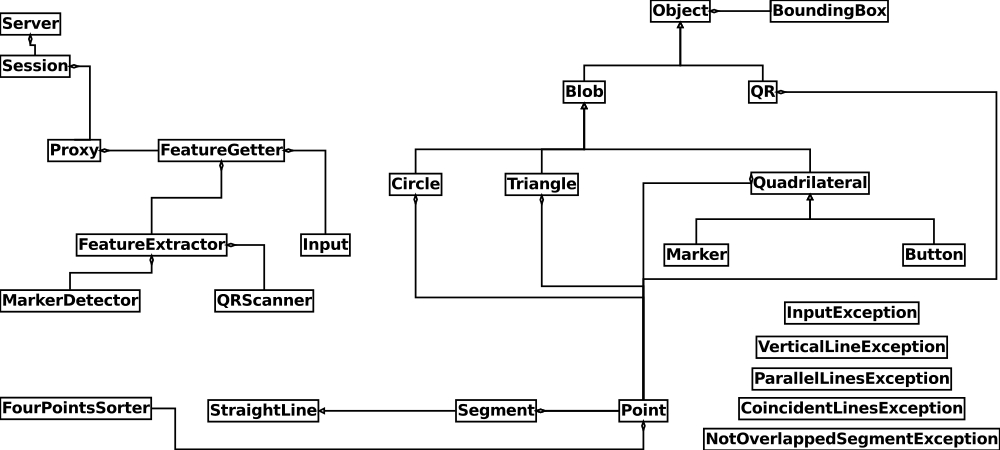
\includegraphics[width=\textwidth*\real{0.9}]{images/ch_06/implementazione_solo_nomi.jpg}
	    }
	  \end{center} 
	  \caption{\textit{Class diagram which illustrates the whole architecture of the software}}  
	  \label{fig:implementationOnlyNames}
 	\end{figure}
 
	Classes \emph{Server} and \emph{Session} manage the communication with \mbox{ACT-R}, implemented by a client server approach.
	Classes \emph{Proxy}, \emph{FeatureGetter}, \emph{Input}, \emph{FeatureExtractor}, \emph{MarkerDetector} and \emph{QRScanner} have the role of extracting the feature from the input data.
	\emph{Object}, \emph{BoundingBox}, \emph{Blob}, \emph{QR}, \emph{Circle}, \emph{Triangle}, \emph{Quadrilateral}, \emph{Marker} and \emph{Button} represent the object hierarchy.
	\emph{InputException}, \emph{NotOverlappedSegmentException}, \emph{ParallelLinesException}, \emph{VerticalLineException}, \emph{CoincidentLinesException}, \emph{FourPointsSorter}, \emph{StraightLine}, \emph{Segment} and \emph{Point} create the utility classes.
	
	Comparing the classes shown in figure \ref{fig:implementationOnlyNames} with the design choices defined in chapter \ref{chDesign}, the reader can notice two facts: both the feature extractor and the class hierarchy parts are composed by the same classes defined in the design and the classes containing the utility functions and the features for the communication with \mbox{ACT-R} have been properly developed, accordingly to the design choices.
	%The following sections presents the implementation of the whole classes, focusing mainly on these two latter parts of the software. 

	\subsection{Feature Extraction}
	
		\begin{figure}[h]
		  \begin{center} 
		    \fbox{	
		       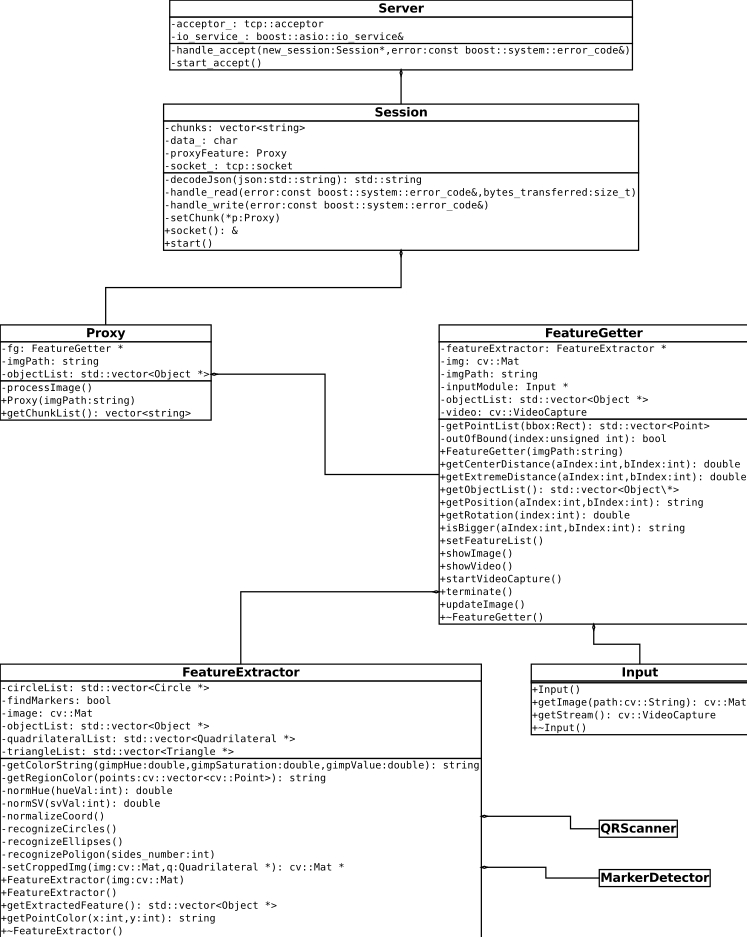
\includegraphics[scale=0.75]{images/ch_06/cs_fe.jpg}
		    }
		  \end{center} 
		  \caption{\textit{}}  
		  \label{fig:extraction and client server}
	 	\end{figure}	


	%\clearpage
 	%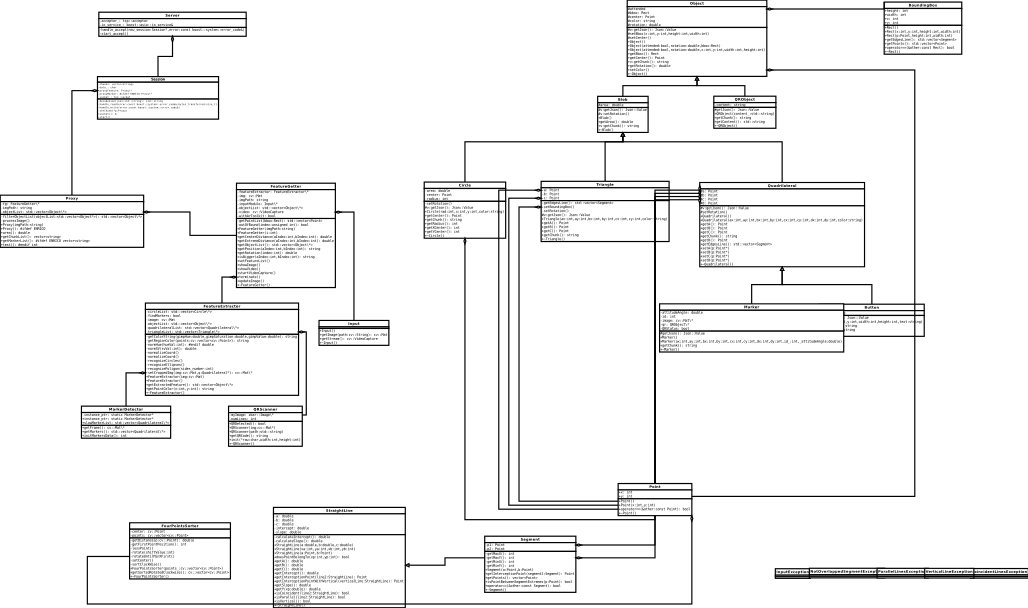
\includegraphics[angle=90,height=\textheight]{images/ch_06/implementation.jpg}\thispagestyle{empty}
\begin{comment}
	\pagestyle{empty}
	\begin{center} 	
	\fbox{	
		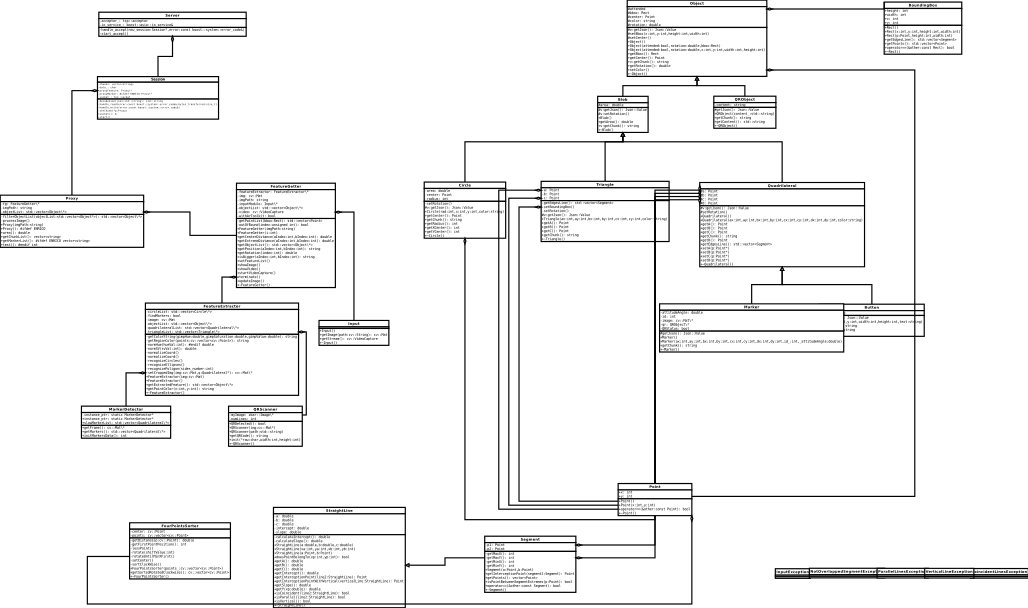
\includegraphics[angle=90,height=26cm]{images/ch_06/implementation.jpg}%\thispagestyle{empty}
	}
	%\caption{\textit{Class diagram illustrating a high level overview of the implementation}} 
	\label{fig:impl}
	\end{center}
\end{comment}
	
	\subsection{Utility Part}
	The utility part is composed by the classes \emph{InputException}, \emph{NotOverlappedSegmentException}, \emph{ParallelLinesException}, \emph{VerticalLineException}, \emph{CoincidentLinesException}, \emph{FourPointsSorter}, \emph{StraightLine}, \emph{Segment}, \emph{Point} and another module containing functions. The latter, as it is not a class, is not included in the diagram in figure \ref{}. 

	\emph{InputException}, \emph{NotOverlappedSegmentException}, \emph{ParallelLinesException}, \emph{VerticalLineException} and \emph{CoincidentLinesException} are exceptions classes, used to handle all the anomalous or exceptional events occurring during the execution of the software. 

	\emph{StraightLine}, \emph{Segment} and \emph{Point} represent geometrical entities. Such elements are fundamental structures for creating the objects in the hierarchy and making evaluations between couples of objects.
	Such evaluations can be both qualitative and quantitative, as, for example, the distances between the centers of tow objects or the relative positions of one object in respect with another.

	\emph{FourPointsSorter} and the function module contain the basic methods which are fundamental for all the operations executed by all the other classes of the software.


	\subsection{Communication with ACT-R}
	The part responsible for the communication with the cognitive architecture is composed by the classes \emph{Server} and \emph{Session}. 
	


 
	\section{Testing}
\begin{comment}

	As it can be seen in the picture, the software is logically divided in the four main components introduced in the design chapter (see \ref{chDesign}).
%, respecting the in the design specifics described in chapter \ref{chDesign}. 
	Both the feature extraction part and the class hierarchy respect the design specifications, described in such chapter. The classes responsible for the communication with \mbox{ACT-R} and the utility part.
The communication with  and


	\newpage
	
	\begin{sidewaysfigure}[hbtp]
	   \thispagestyle{empty}	
 	   \centering
	   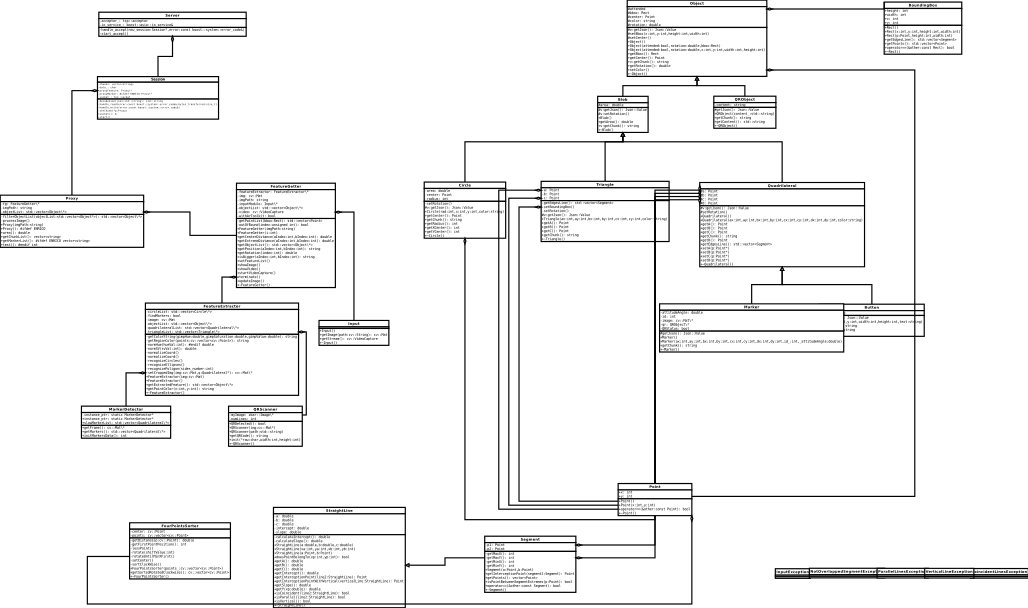
\includegraphics[height=\textheight]{images/ch_06/implementation.jpg}
	   
	  \caption{\textit{Class diagram illustrating the class hierarchy of the recognized objects}}  
	  \label{fig:HierarchyDesign}
 	\end{sidewaysfigure}

\newpage

\relax
	\AddToShipoutPicture*{ \\ \relax
	  \setlength{\unitlength}{1mm} 
	  \put(<10>, <10>){  
	    \makebox(0,0){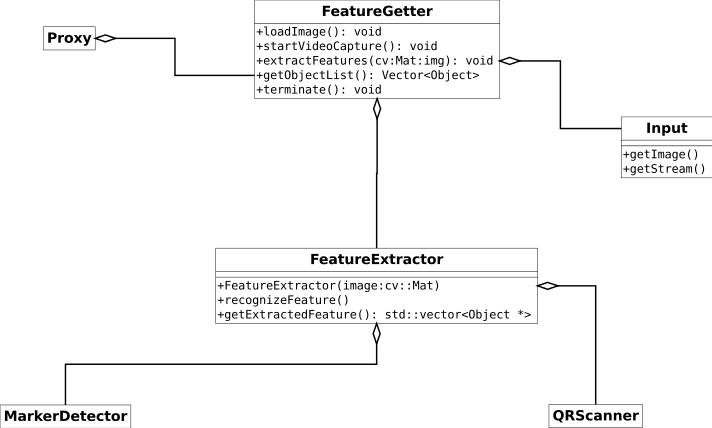
\includegraphics{images/ch_05/feature.png}}}} 
	ciao

	
\end{comment}

	%\section{COmmunication with ACT-R}
	%ciao
